\frame{
  \frametitle{Definições}
  \begin{block}{}
    \begin{figure}
      \centering
      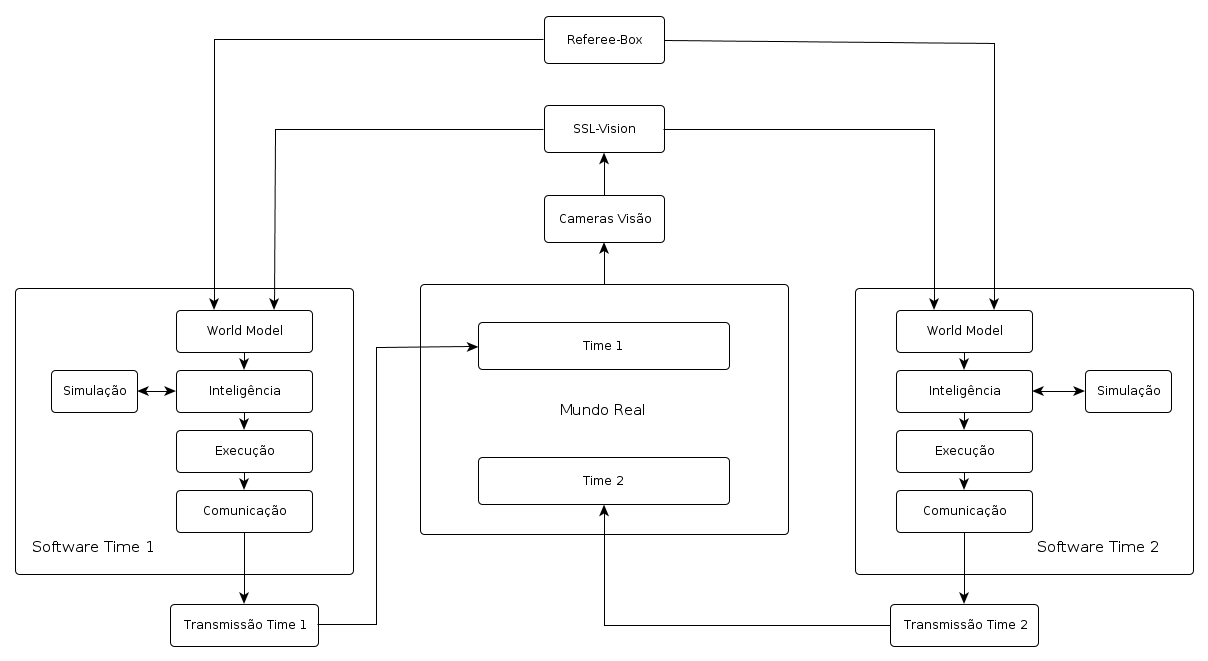
\includegraphics[width=9cm]{imgs/arquitetura_ssl}
      \caption{Arquitetura básica da SSL}
    \end{figure}
  \end{block}
}

\frame{
  \frametitle{Definições}
    \begin{block}{}
    \begin{figure}
      \centering
      \includegraphics[width=7cm]{imgs/corpo_rigido}
      \caption{Modelo um Corpo Rígido}
    \end{figure}
  \end{block}
}

\frame{
  \frametitle{Definições}
    \begin{block}{}
    \begin{figure}
      \centering
      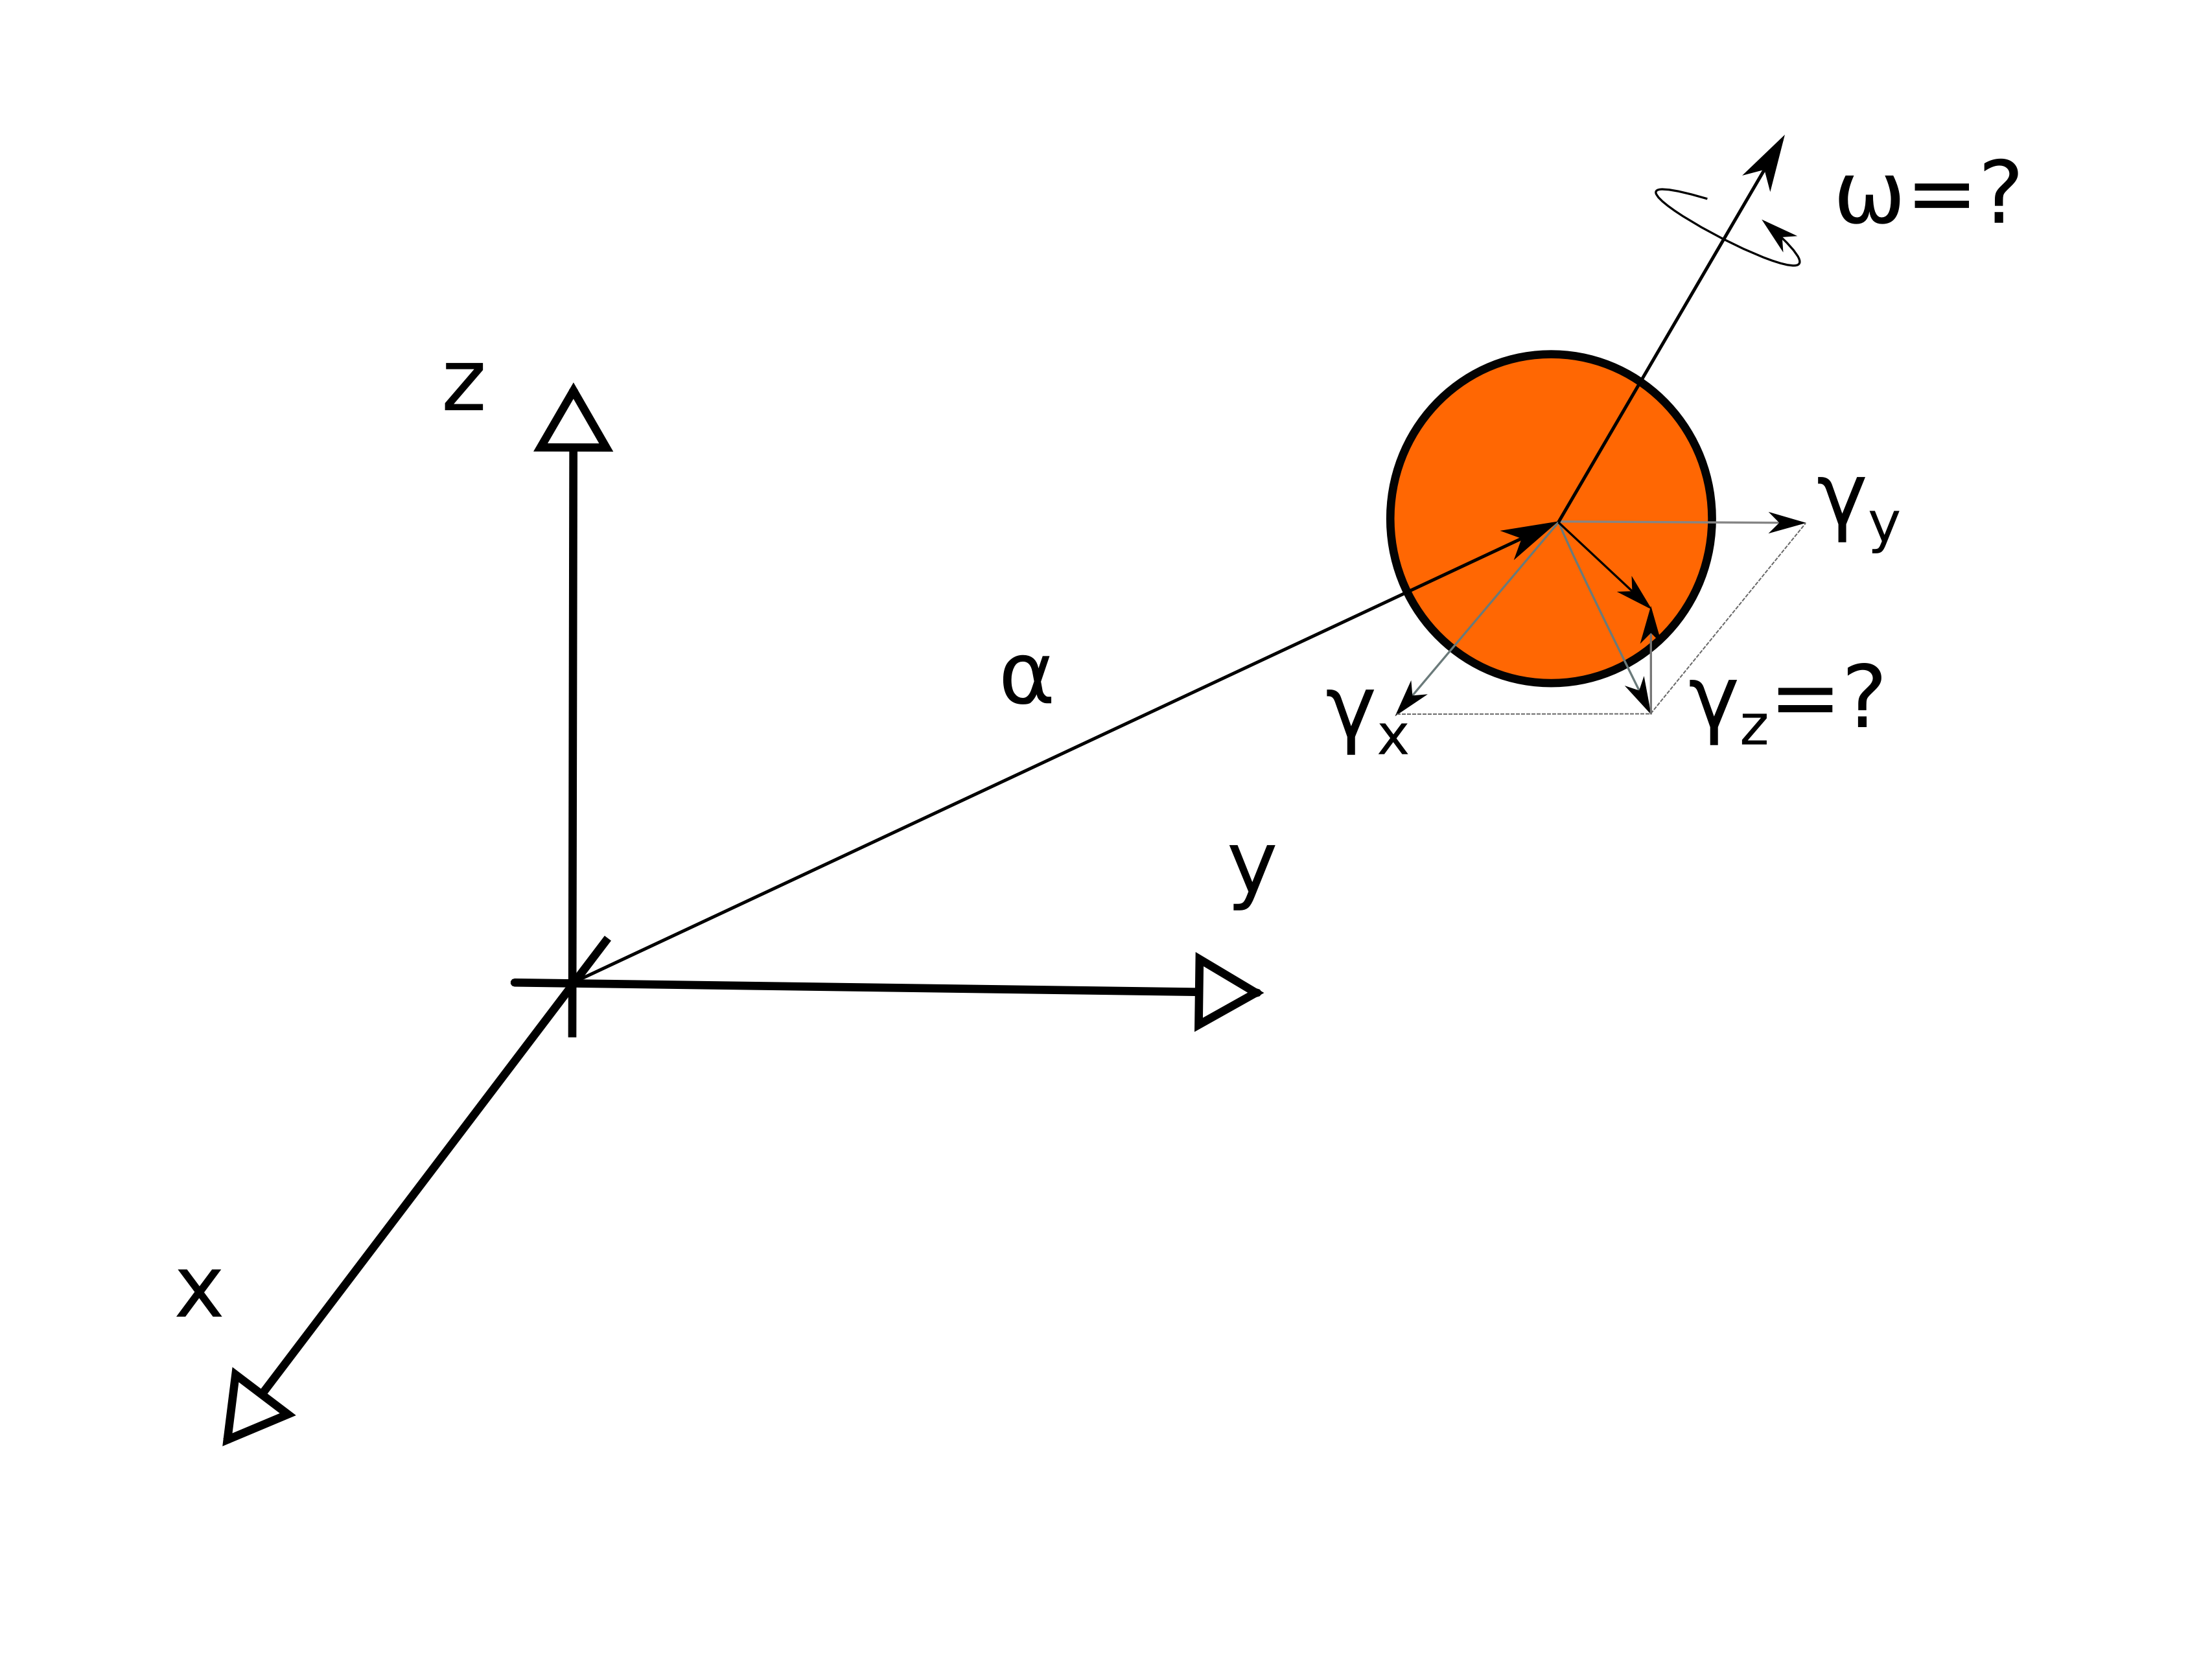
\includegraphics[width=6cm]{imgs/bola}
      \caption{Modelo da Bola}
    \end{figure}
  \end{block}
}

\frame{
  \frametitle{Definições}
    \begin{block}{}
    \begin{figure}
      \centering
      %------------PRIMEIRA FIGURA------------------
      \begin{minipage}[b]{0.4\linewidth}
        \centering
        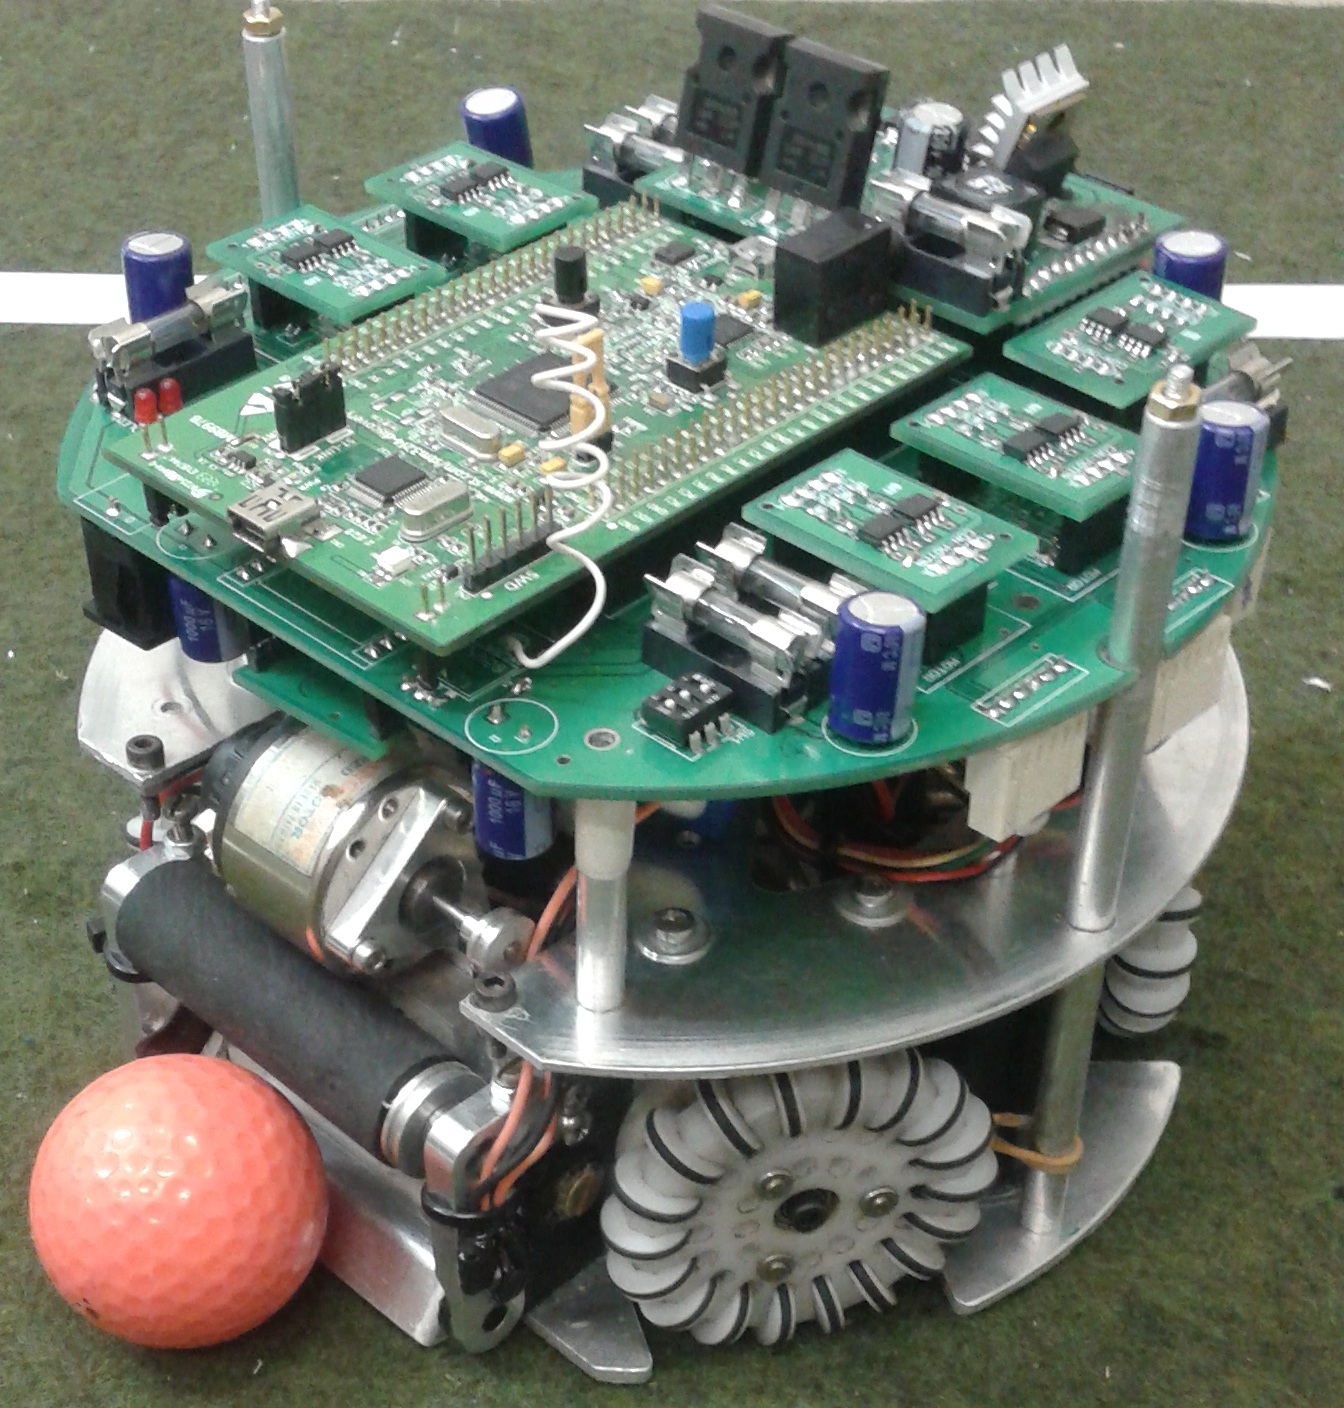
\includegraphics[width=\linewidth]{imgs/real}
        \caption{Robô Real}
      \end{minipage}
      %---------------------------------------------
      \hfill
      %-------------SEGUNDA FIGURA------------------
      \begin{minipage}[b]{0.4\linewidth}
        \centering
        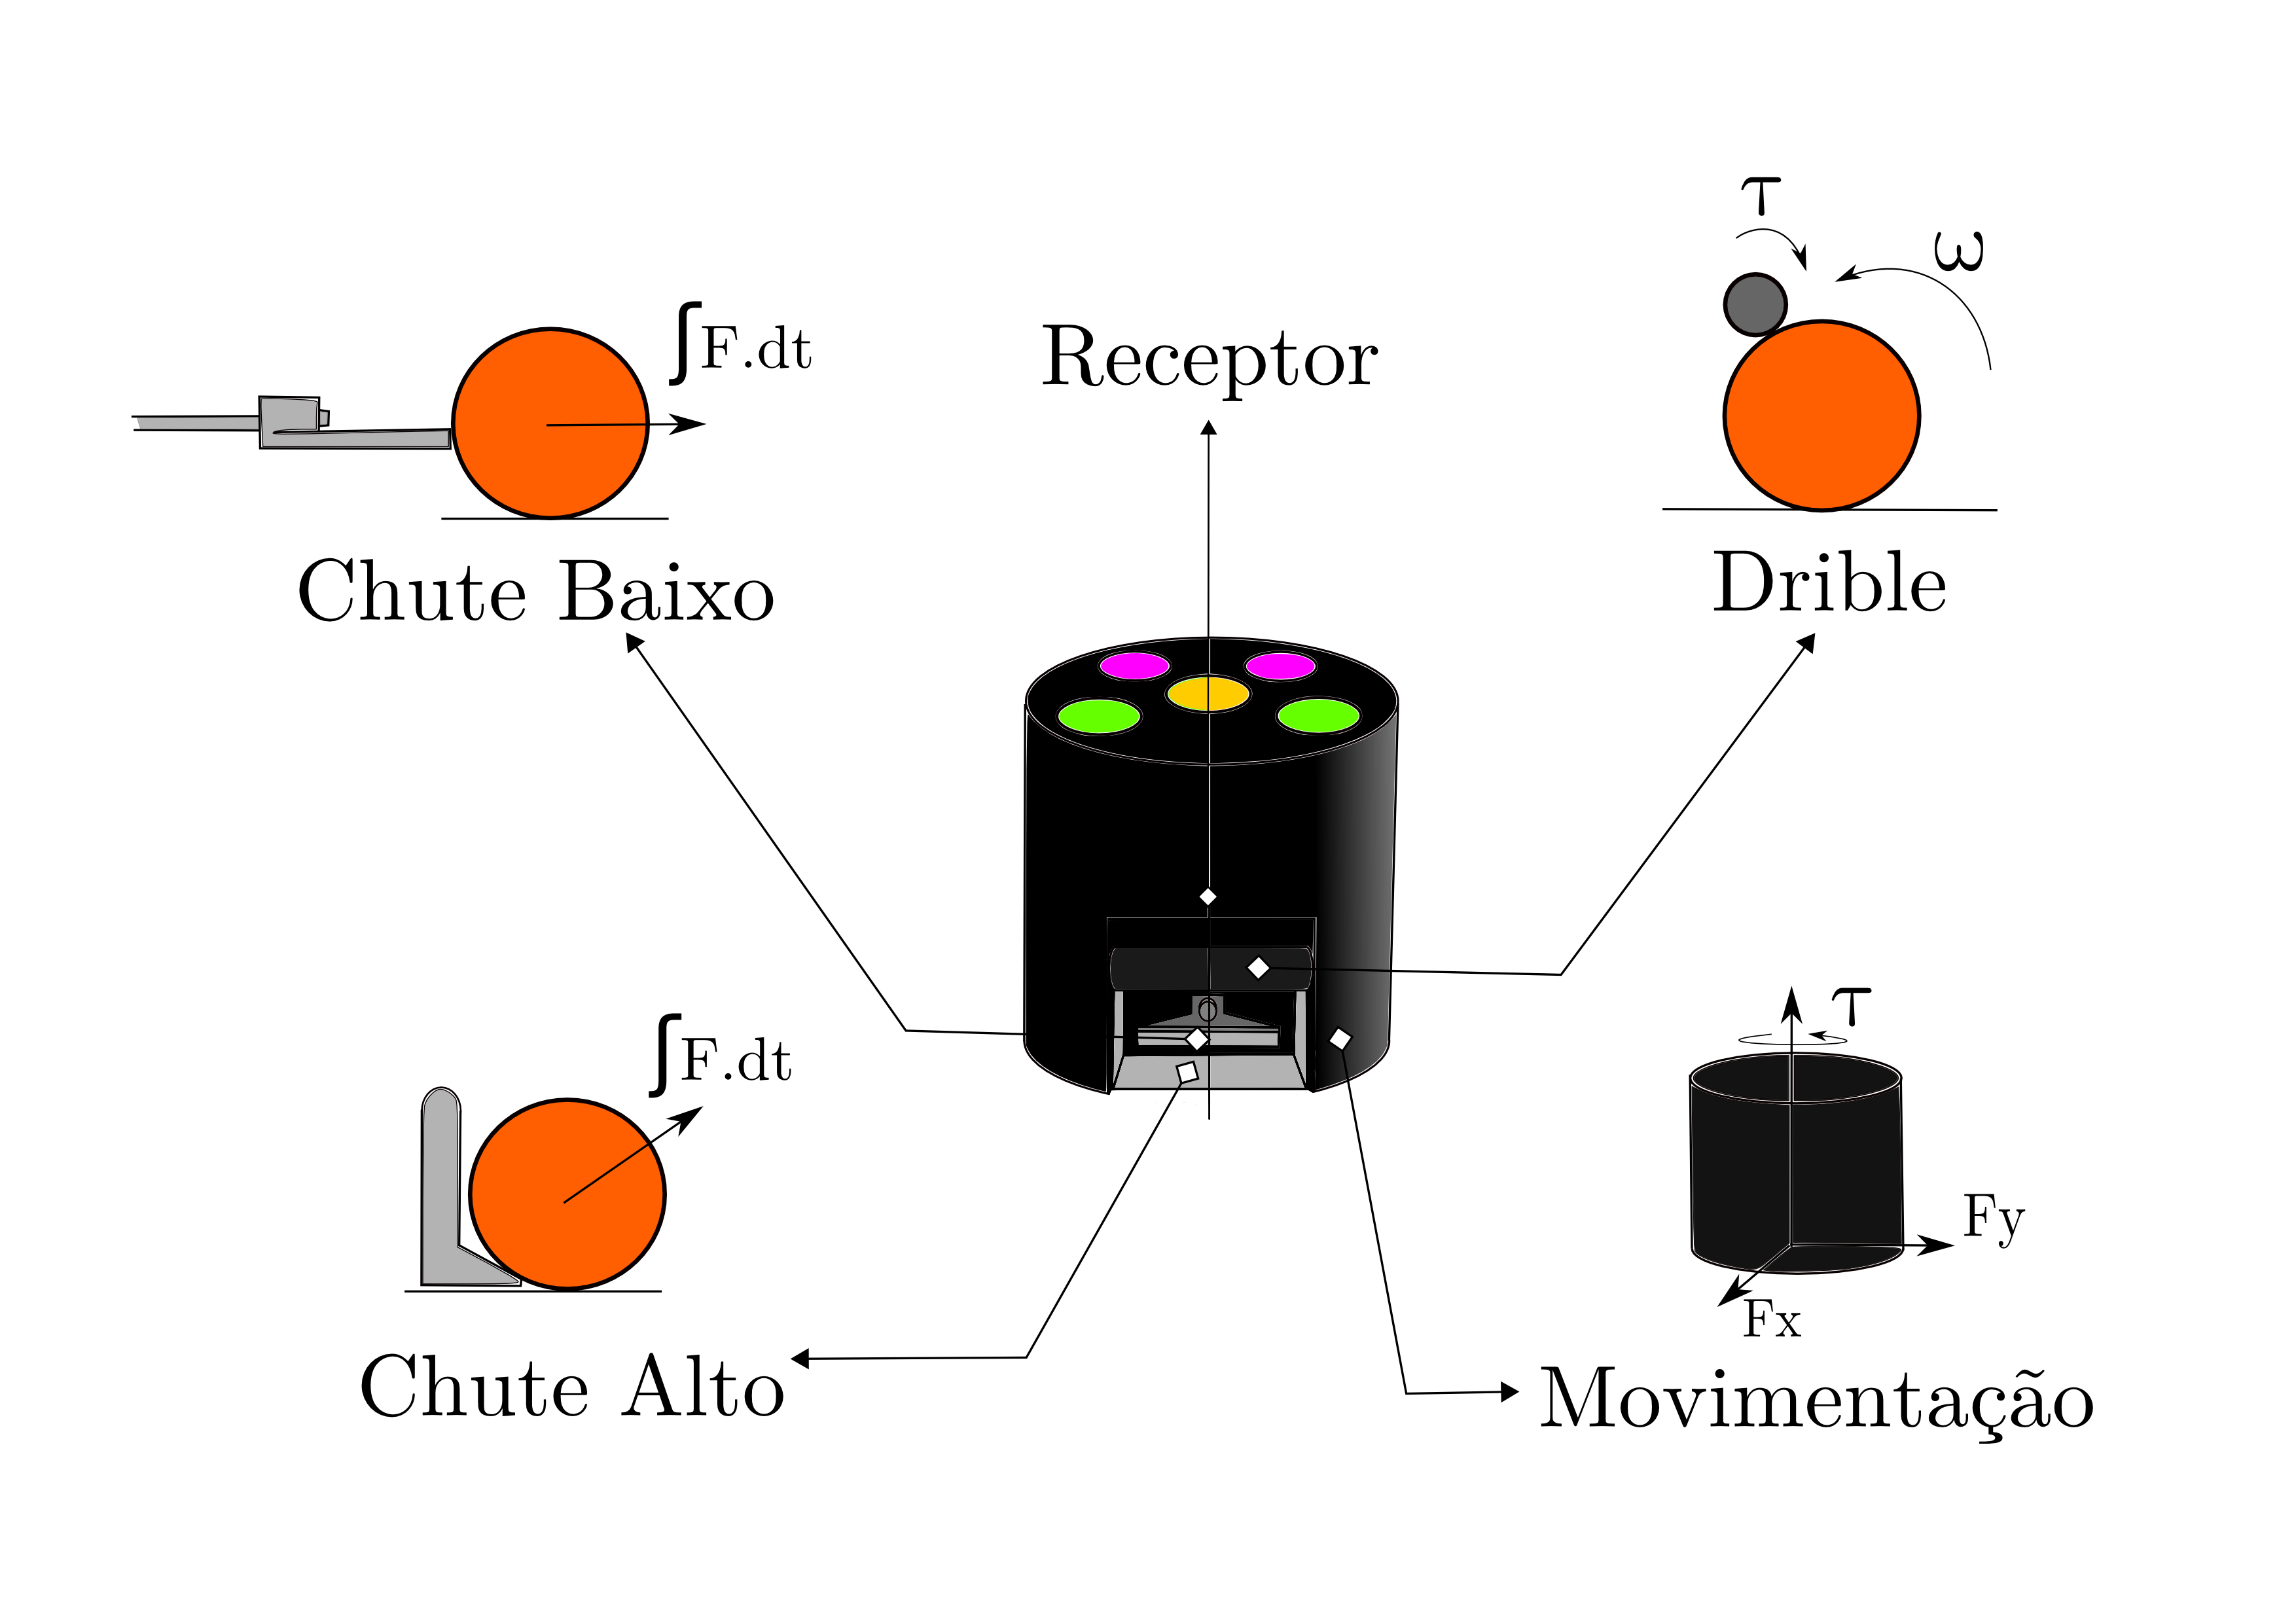
\includegraphics[width=\linewidth]{imgs/robo}
        \caption{Modelagem do Robô Real}
      \end{minipage}
    \end{figure}
  \end{block}
}

\frame{
  \frametitle{Definições}
    \begin{block}{}
    \begin{figure}
      \centering
      \includegraphics[width=4.5cm]{imgs/time_robocup}
      \caption{Partida da SSL Robocup 2013}
    \end{figure}
  \end{block}
  \begin{block}{}
    \textbf{Time} 
    \[T: \langle A, X_{ob}^{i},e,e_b,r_i \rangle \rightarrow 
    a_c^{i+1}\]
  \end{block}
}

\frame{
  \frametitle{Definições}
    \begin{block}{}
      \textbf{Partida} $p=$
      \[ \lbrace T_1, T_2, \Delta t, \delta t, \langle
      Ref^{0}, Xob^{0}, A_1^{0}, A_2^{0},\rangle, \cdots ,
      \langle Ref^{N}, Xob^{N}, A_1^{N}, A_2^{N}
      \rangle \rbrace \]
    \end{block}
    
    \begin{block}{}
      \textbf{Log}
      \[log(p) = \lbrace p.\langle Ref^{0}, X_{ob}^{0}\rangle,
      \cdots, \lbrace p.\langle Ref^{0}, X_{ob}^{0}\rangle
      \rbrace \]
    \end{block}
}